\documentclass{article}
\usepackage{imakeidx}
\usepackage{multirow}
\usepackage[a4paper,top=2cm,bottom=2.5cm,left=1.5cm,right=1.5cm,marginparwidth=1.75cm]{geometry}
\usepackage{amsmath}
\usepackage{graphicx}
\usepackage{subfig}
\usepackage{caption}
\usepackage{geometry}
\usepackage{datetime}
\usepackage{wrapfig}
\usepackage[T1]{fontenc}
\usepackage[utf8]{inputenc}
\usepackage[portuguese]{babel}
\usepackage{hyphenat}
\usepackage[export]{adjustbox}
\usepackage[colorlinks=true, allcolors=black]{hyperref}
\usepackage{comment}
\usepackage{blindtext}
\usepackage{graphicx}
\usepackage{float}
\usepackage{tablefootnote}
\usepackage[bottom]{footmisc}
\usepackage[table,xcdraw]{xcolor}
\usepackage{subfig}
\usepackage[utf8]{inputenc}
\usepackage{graphicx}

\begin{document}
\begin{center}
    \begin{minipage}{0.83\linewidth}
        \centering
        
\includegraphics[width=0.4\textwidth]{Images/UM.jpg}\par\vspace{0.5cm}
        {\scshape\textbf{Universidade do Minho}} \par
        {\scshape Licenciatura em Engenharia Informática} \par
        \vspace{3cm}
        {\LARGE Fase 1\\} \par
        {\scshape\LARGE \textbf{Projeto LI3}\\} \par
        \vspace{1.0cm}
        {\LARGE \textbf{Airline Manager}} \par
        \vspace{2cm}
        {\LARGE\textbf {PL6 - Grupo 27}} \par
        \vspace{0.1cm}
        {\LARGE Hugo Abelheira(a95151)\par Luís França(a104259)\par Mariana Rocha(a90817) \par}
        
        \vspace{5cm}
        {\large \today\par}
        
    \end{minipage}
\end{center}
\newpage
\tableofcontents
\listoffigures

\newpage
\section{Introdução}
\paragraph{}O projeto em desenvolvimento no âmbito da disciplina de Laboratórios de Informática 3 tem como objetivo principal realizar o tratamento de dados provenientes de extensos conjuntos de informações contidas em arquivos CSV. Este tratamento envolve a implementação de um processo de parsing, onde os dados são interpretados e transformados em entidades representativas, que por sua vez são armazenadas em estruturas de dados específicas denominadas catálogos.
\vspace{-0.75cm} %idk why but needed more space
\paragraph{}Além do \textit{parsing}, uma etapa crítica do projeto envolve a validação de campos, garantindo a integridade e consistência dos dados processados.
\vspace{-0.3cm}
\paragraph{}Os catálogos criados não apenas armazenam os dados de maneira eficiente, mas também servem como base para a execução de \textit{queries} (consultas). Utilizando diversas estruturas de dados adicionais, o projeto propõe a implementação de \textit{queries} que fornecem informações específicas a partir dos dados armazenados nos catálogos. Estas são formuladas com base em requisitos pré-definidos e, quando executadas, geram resultados que são posteriormente processados e apresentados no respetivo formato.
\vspace{-0.3cm}  
\paragraph{}A complexidade do projeto é ampliada pelo facto de nos ser fornecido um ficheiro de \textit{input}, onde cada linha contém um comando que corresponde ao tipo da \textit{query} e os argumentos associados. A execução desses comandos requer uma lógica adaptativa, garantindo que cada \textit{query} seja processada corretamente e que os resultados sejam armazenados nos respetivos ficheiros de \textit{output}.
\vspace{-0.3cm}
\paragraph{}Dessa forma, este projeto abrange uma variedade de conceitos essenciais, funcionando também como uma ponte de aprendizagem para programação orientada a objetos, desde manipulação de arquivos e \textit{parsing} de dados até a manipulação de estruturas de dados complexas e a execução dinâmica de consultas. O desafio reside não apenas na correta implementação desses aspetos individuais, mas também na integração eficiente e eficaz de todos os elementos para criar um sistema coeso e funcional.

\section{Arquitetura do Projeto}
\paragraph{}Ao conceber a arquitetura deste projeto, adotamos uma abordagem modular para garantir uma implementação robusta e escalável. O sistema é composto por vários módulos relacionados entre si, cada um responsável por tarefas diferentes, mas resumidamente dividos em 3 componentes essenciais: \textbf{Processamento de Entrada}, \textbf{Lógica de Negócios} e \textbf{Geração de Resultados}.

\subsection{Processamento de Entrada}
\paragraph{}Os módulo encarregues pelo Processamento de Entrada são responsáveis pela ingestão de dados brutos provenientes de arquivos CSV. Nesta fase, os dados são submetidos a um processo de \textit{parsing}, onde são extraídas informações relevantes e validadas quanto à integridade dos campos. Durante esse processo, as entidades são construídas e os dados são transformados para serem armazenados nos catálogos correspondentes. Há ainda um módulo extra nesta componente inicial chamado \textit{interpreter} que tem a mesma função que o \textit{parser} mas para o ficheiro de \textit{input}, que contém um comando por linha, onde cada comando corresponde à execução de uma \textit{query}.

\subsection{Lógica de Negócios}
\paragraph{}A Lógica de Negócios representa o núcleo do sistema, onde os catálogos são continuamente alimentados e atualizados. Utilizamos a biblioteca \textit{GLib} para criar estruturas de dados dinâmicas que se ajustam às necessidades variáveis do projeto. A validação contínua dos dados durante o processo de \textit{parsing} assegura a coerência dos catálogos. 
Num módulo \textit{interpreter} identificamos o tipo de \textit{query} que queremos executar e, utilizando as informações contidas nos catálogos (gerenciadas por um \textit{catalog manager}, que corresponde à operação lógica de junção de todos os outros catálogos), um outro módulo \textit{queries} resolve a \textit{query} em questão, produzindo os resultados correspondentes para a escrita do \textit{output} correspondente.

\subsection{Geração de Saída}
\paragraph{}O módulo de Geração de Saída chamado \textit{output}, é responsável por criar os resultados das \textit{queries} em ficheiros de texto. Durante a execução das \textit{queries}, os resultados são formatados como pedido e armazenados de maneira eficiente nos arquivos de saída, preservando a estrutura e integridade dos dados. Esta fase utiliza as estruturas de dados previamente construídas nos catálogos.

\subsection{Representação Visual}
\paragraph{}A Figura 1 apresenta um diagrama simplificado que ilustra as principais classes e suas interações no sistema. Este diagrama proporciona uma visão visual clara da estrutura do projeto.
\begin{figure}[H]
\begin{center}
	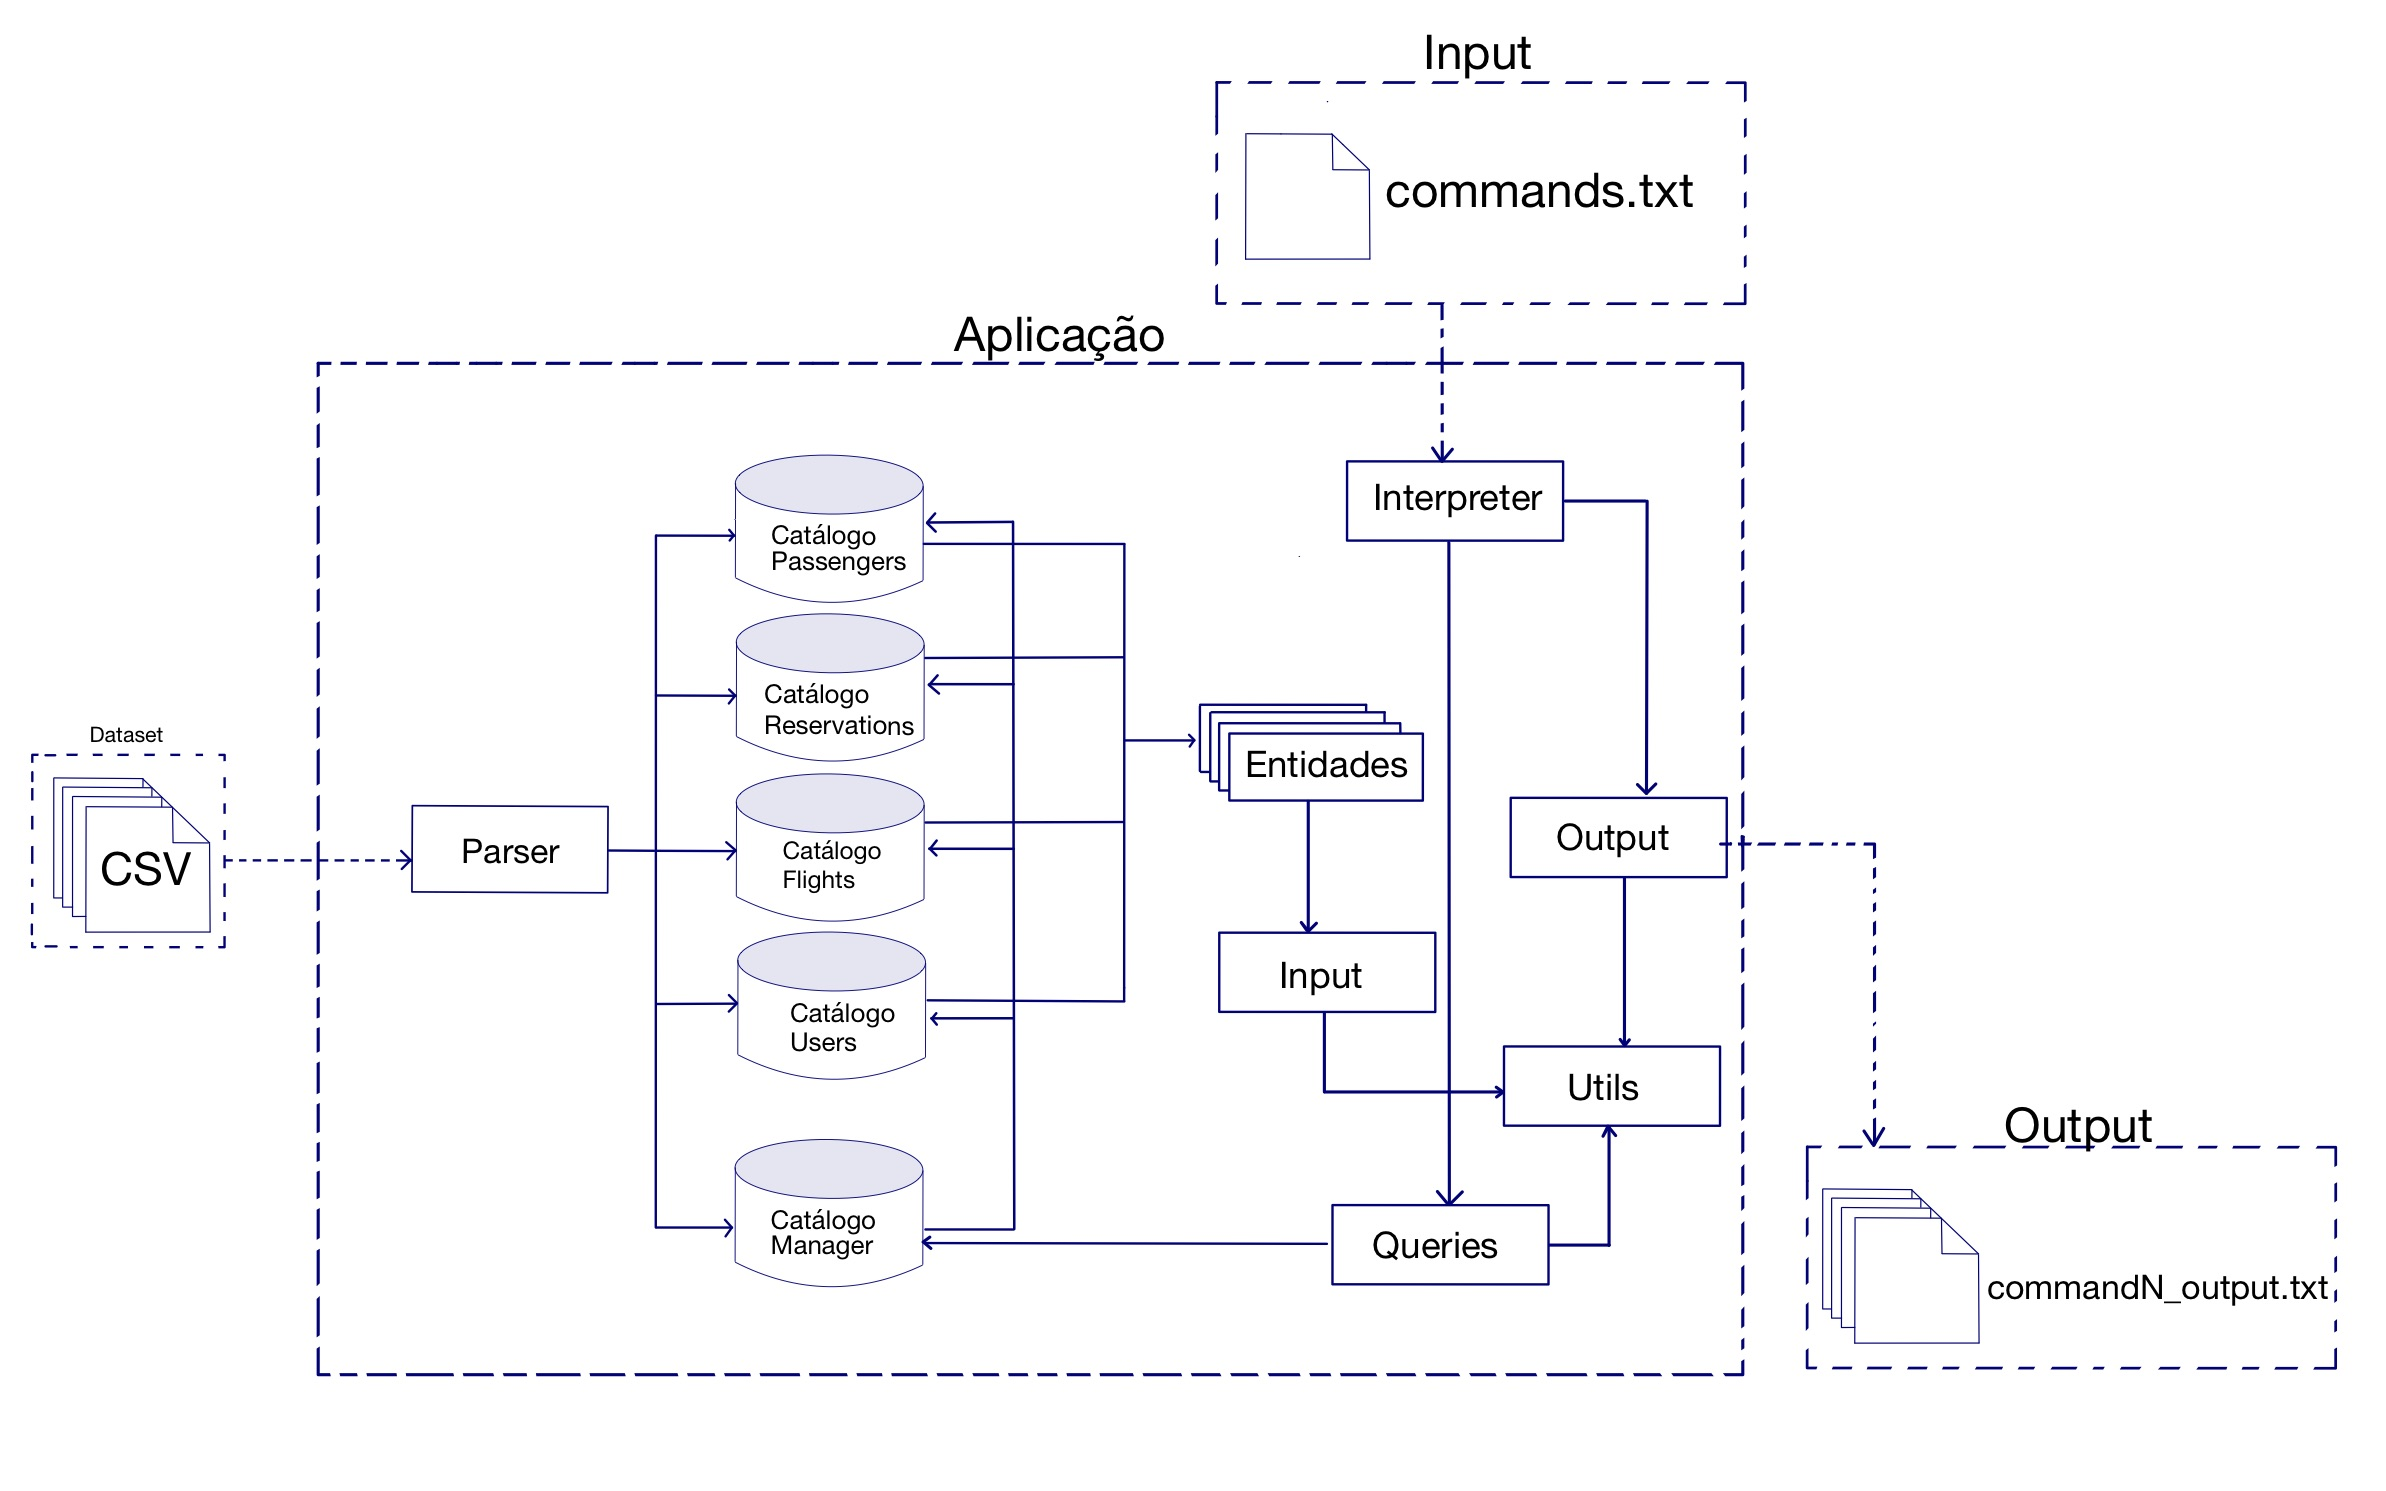
\includegraphics[width=15cm]{Images/arquitetura.png} 
        \caption{Representação da Arquitetura do Projeto}
\end{center}
\end{figure}

\subsection{Considerações de Desempenho e Escalabilidade}
\paragraph{}A arquitetura foi projetada com ênfase na eficiência do processamento, minimizando a complexidade temporal e espacial. Utilizamos estruturas de dados dinâmicas, fornecidas pela biblioteca \textit{GLib}, o que garante escalabilidade e permite a gestão eficaz de grandes conjuntos de dados. 

\subsection{Padrões e Tecnologias Utilizados}
\paragraph{}Optamos por adotar uma abordagem modular na organização do código-fonte, dando prioridade à criação de módulos específicos à medida que identificamos conjuntos de funções com complexidade suficiente para justificar um novo módulo. Essa abordagem favorece a clareza e a manutenção do código, permitindo que cada módulo tenha responsabilidades bem definidas e uma interface coesa.

\subsection{Configuração e Compilação}
O \textit{Makefile} desempenha um papel crucial na organização e automatização do processo de compilação do nosso projeto. Este arquivo de configuração não só simplifica a construção do código-fonte, mas também facilita a manutenção e distribuição do projeto.
Alguns aspetos importantes a considerar sobre o nosso \textit{Makefile} são:
\begin{itemize}
\vspace{-0.2cm}
\item As flags de compilação incluem opções específicas para a biblioteca GLib, garantindo a compatibilidade e correta ligação durante o processo de compilação.
\item O Makefile suporta dois modos distintos de compilação: Debug e Release.
\item A estrutura do projeto é mantida através da criação de diretórios conforme necessário durante o processo de compilação.
\item Integrado ao Makefile, temos suporte para a geração automática de documentação usando o Doxygen.
\item O Makefile inclui uma regra "clean" para remover todos os objetos e ficheiros gerados durante o processo de compilação.
\end{itemize}

\subsection{Conclusão}
\paragraph{}A arquitetura proposta fornece uma base sólida para a implementação do projeto, garantindo a modularidade, a eficiência e a facilidade de manutenção. A interconexão fluida entre os módulos permite que o sistema atenda de forma eficaz aos requisitos funcionais, ao mesmo tempo que mantém a flexibilidade necessária para futuras expansões e melhorias.

\section{Desenvolvimento e Ideias Iniciais}
\paragraph{}Antes de entrar nos detalhes sobre o desenvolvimento do \textit{parser}, é relevante destacar a importância do \textit{makefile} e da validação de dados na fase inicial do projeto.

\paragraph{}O \textit{makefile} foi concebido como uma ferramenta fundamental para a automatização do processo de compilação. Ele não apenas organizou a estrutura do projeto, facilitando a compilação e vinculação de diferentes módulos, mas também permitiu uma abordagem mais eficiente para gerir dependências e garantir a integridade do código.

\paragraph{}A validação de dados, por sua vez, tornou-se um ponto fulcral durante o desenvolvimento. A garantia da qualidade e consistência dos dados foi estabelecida como uma prioridade. Essa fase inicial envolveu a implementação de mecanismos de verificação rigorosos para assegurar que o \textit{dataset} estivesse em conformidade com as expectativas do sistema. Isso não apenas contribuiu para a estabilidade do código, mas também preveniu potenciais problemas ao longo das etapas subsequentes do desenvolvimento. 

\paragraph{}Após a definição da arquitetura do projeto, focamo-nos no desenvolvimento do código, iniciando com a implementação de um \textit{parser} para os ficheiros \textit{CSV}. O \textit{parser} desempenhou um papel crucial ao formatar as linhas do ficheiro em campos separados. Vale destacar que o \textit{parser} não executa validações diretamente; em vez disso, é nesse ponto que chamamos as funções específicas de validação, tornando o processo mais modular e compreensível.

\paragraph{}Dando continuidade, introduzimos o módulo \textit{batch}, uma peça fundamental que não só encaminhava os argumentos essenciais para as funções de \textit{parsing}, mas era também responsável por chamar o módulo \textit{interpreter} que por sua vez lê o ficheiro de \textit{input}.

\paragraph{}Com os mecanismos de \textit{parsing} consolidados, passamos à criação de estruturas de dados dedicadas para armazenar as informações dos ficheiros \textit{CSV}. Introduzimos catálogos específicos para cada tipo de ficheiro, como passageiros, voos, utilizadores e reservas. Esses catálogos foram implementados como \textit{hash tables} proporcionando um acesso rápido e eficiente aos dados. Nesta fase, adotamos uma estratégia que nós pensamos ser bastante interessante. Deparámo-nos com um erro ao associar a  \textit{string id} com a instância da entidade. Para isso, criamos vários \textit{pointer arrays} (estrutura da \textit{GLib} que representa um \textit{array} dinâmico) para podermos associar uma chave criada por nós (um valor inteiro) ao respetivo \textit{string id}. Depois criamos ainda \textit{hash tables} extra para podermos associar a \textit{string id} à chave criada por nós.

\paragraph{}Ao avançar para a fase de execução de \textit{queries}, desenvolvemos um sistema capaz de analisar e executar \textit{queries}, gerando resultados que eram registados em ficheiros de saída designados por \textit{commandN\_output.txt} (onde N identifica o número da linha do ficheiro de \textit{input}). 

\paragraph{}Na escolha das \textit{queries} a serem implementadas na primeira fase, optamos por aquelas que consideramos mais viáveis dentro do cronograma estabelecido. Por fim, conferimos atenção meticulosa à gestão de memória, garantindo não apenas a alocação adequada, mas também a libertação eficiente de todos os espaços alocados ao longo do programa, evitando assim possíveis \textit{memory leaks}, um desafio que enfrentamos e superamos ao longo do processo de desenvolvimento. Exploramos mais aprofundadamente numa secção seguinte estes \textit{memory leaks} e a sua resolução.

\section{Soluções e Resolução de problemas}
\paragraph{}Durante a fase de \textit{parsing}, implementamos uma abordagem inicial, mas ao longo do desenvolvimento, percebemos a necessidade de ajustes para resolver questões específicas, tais como a criação dos ficheiros de erro neste processo, invés de serem criados mais tarde. 

\paragraph{}A validação do \textit{dataset} e a criação de entidades foram etapas críticas. Enfrentamos desafios relacionados com o encapsulamento, garantindo que as cópias fossem tratadas de maneira apropriada. Além disso, a alocação de memória foi cuidadosamente gerenciada para evitar \textit{memory leaks}, e a construção adequada de entidades foi crucial para garantir o comportamento desejado do sistema.

\paragraph{}A implementação dos catálogos representou uma das fases mais desafiadoras do projeto. Inserir informações de maneira correta e sem provocar \textit{memory leaks} exigiu uma atenção minuciosa. Enfrentamos diversos problemas inesperados, tais como, o \textit{insert} das entidades, que não era identificado como erro, no entanto estava a preencher as nossas bases de dados com lixo, tornando este um erro bastante difícil de identificar, que foi apenas óbvia quando identificamos outro erro quando tentamos libertar a memória alocada para os catálogos. No entanto, a resolução desses desafios proporcionou aprendizagens valiosas, resultando em soluções tanto otimizadas quanto aquelas que nos ensinaram a lidar com obstáculos inesperados.

\paragraph{}A etapa de \textit{queries} foi mais complexa do que inicialmente prevíamos. Muitos dos problemas encontrados estavam relacionados aos catálogos ou ao comportamento inesperado de certas estruturas de dados e funções da \textit{GLib}. No entanto, encontrar as estratégias que nos permitissem não só executar as \textit{queries} de forma eficiente mas também poder ter acesso a informação que se encontra noutros módulos, foi demorado e apresentou o seu grau de complexidade. Superar esses desafios contribuiu para uma compreensão mais profunda do funcionamento do sistema e aprimorou a robustez do código.
%complexidade aka torturante

\paragraph{}Finalmente, ao encontrar uma solução eficaz para utilizar o \textit{array result}, a implementação da geração de ficheiros de \textit{output} tornou-se uma tarefa relativamente simples. Essa escolha estratégica facilitou o processo de desenvolvimento e proporcionou uma conclusão bem-sucedida para o projeto, destacando a importância de escolhas estruturais na resolução de desafios técnicos.

\subsection{Valgrind & Debugger (GDB)}
\paragraph{}Para validar a correta execução do programa, utilizamos as ferramentas de depuração Valgrind e GDB. Apesar de distintas, essas ferramentas se complementam no processo de identificação e correção de erros. O Valgrind concentra-se principalmente em detectar \textit{memory leaks} (quando um programa aloca memória dinamicamente, mas não a libera adequadamente, resultando em desperdício de recursos de memória) e acessos indevidos (quando um programa tenta ler ou escrever em áreas de memória não alocadas para ele, podendo levar a comportamentos indesejados, falhas ou \textit{crashes}) durante a execução do programa. Por sua vez, o GDB contribui para esse propósito, permitindo a criação de pontos de interrupção (\textit{breakpoints}), nos quais podemos acessar os valores das variáveis do programa e realizar \textit{backtrace} para localizar a origem de um problema.

\subsubsection{Guia de Utilização das Ferramentas}
Para poder utilizar o GDB temos que executar os seguintes comandos:
\begin{itemize}
\item gdb ./programa-principal
\item run <path\_datasets> <path\_ficheiro\_input>/input.txt
\end{itemize}
Para poder utilizar o Valgrind temos que executar os seguintes comandos:
\begin{itemize}
\item valgrind ./programa-principal <path\_datasets> <path\_ficheiro\_input>/input.txt
\vspace{0.1cm}
\par Ou para uma análise mais detalhada...
\item valgrind —leak-check=full ./programa-principal <path\_datasets> <path\_ficheiro\_input>/input.txt
\end{itemize}
\paragraph{}É ainda importante mencionar que o projeto deve ser compilado antes de aceder a qualquer uma das ferramentas, através do comando make. Ainda podemos utilizar a \textit{flag DEBUG=1} para obter informações mais específicas sobre o erro.

\paragraph{}Nas figuras que se seguem, podemos ver como é que o \textit{Valgrind} nos mostra a quantidade de \textit{memory leaks} que temos no projeto. Inicialmente identificamos imensos vazamentos durante a criação dos catálogos. É de notar que a quantidade de \textit{memory leaks} inicial Figura\ref{Figura1Valgrind} não representa todos os possíveis vazamentos, antes de obter os 23 \textit{MegaBytes} resolvemos outras imensas \textit{leaks}.
\begin{figure}[H]
\begin{center}
	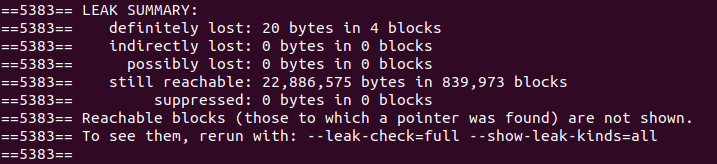
\includegraphics[width=15cm]{Images/valgrindPior.png} 
        \caption{Quantidade de \textit{memory leaks} inicial}
        \label{Figura1Valgrind}
\end{center}
\end{figure}
\paragraph{}Depois de completados os catálogos, o desenvolvimento das \textit{queries} foi a etapa mais problemática pois, mesmo que a quantidade de \textit{leaks} seja menor, a sua resolução foi bastante mais complexa, pois mesmo identificando os locais corretos cuja memória necessitava de ser libertada, era muito fácil deixar alguns apontadores alocados ou então dar \textit{free} duplicados. 
\begin{figure}[H]
\begin{center}
	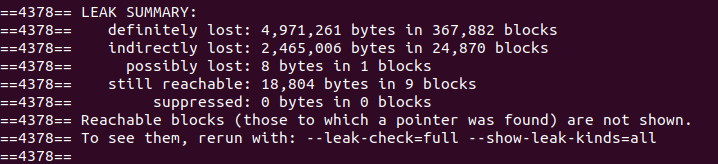
\includegraphics[width=15cm]{Images/valgrindMédio.png} 
        \caption{Quantidade de \textit{memory leaks} otimizada}
        \label{Figura2Valgrind}
\end{center}
\end{figure}
\paragraph{}Na fase final, conseguimos otimizar bastante o nosso código, não só em \textit{memory leaks} como também em memória total usada e tempo de execução. Infelizmente continuamos ainda com 100 \textit{Bytes} de memória perdida, porque mesmo com o problema identificado, a estratégia que usamos para resolver os restantes \textit{leaks} não resultou aqui. Estamos confiantes que na próxima fase serão resolvidos.
\begin{figure}[H]
\begin{center}
	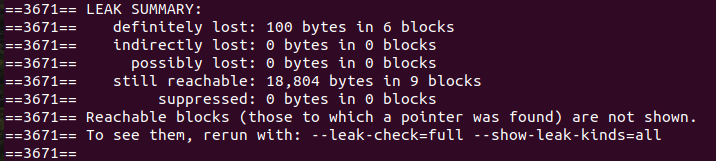
\includegraphics[width=15cm]{Images/valgrindMelhor.png} 
        \caption{Quantidade de \textit{memory leaks} final}
        \label{Figura3Valgrind}
\end{center}
\end{figure}
\newpage
\section{Resultados Finais}
\paragraph{}\textit{Query 1}: “Listar o resumo de um utilizador, voo, ou reserva, consoante o identificador recebido por argumento.”
A função \textit{query1} foi criada para extrair informações com base em um ID de entidade, que pode representar um voo, uma reserva ou um usuário, dependendo das condições de identificação. Ao receber um \textit{ID} como argumento, a função verifica se corresponde a um voo, reserva ou usuário, utilizando funções de obtenção específicas. Se a correspondência for encontrada, a função coleta informações pertinentes, como detalhes do voo, reserva ou usuário, e retorna um \textit{array} de strings dinamicamente alocado contendo esses dados. Além disso, a função faz a gestão adequada da memória, libertando-a quando necessário, e trata casos especiais, como usuários inativos, retornando \textit{NULL} nessas situações.
\paragraph{}\textit{Query 2}: “Listar os voos ou reservas de um utilizador, se o segundo argumento for \textit{flights} ou \textit{reservations}, respetivamente, ordenados por data (da mais recente para a mais antiga). Caso não seja fornecido um segundo argumento, apresentar voos e reservas, juntamente com o tipo (\textit{flight} ou \textit{reservation}).”
A função \textit{query2} é projetada para extrair informações relacionadas a voos e reservas associados a um usuário, permitindo a filtragem por tipo (todos, voos ou reservas) e a ordenação por data e identificador. A função utiliza estruturas de dados, como \textit{ResultEntry}, para representar informações de resultados, e implementa funções de comparação para ordenação. Ela manipula dinamicamente \textit{arrays} de \textit{IDs}, datas e tipos, iterando sobre voos e reservas associados ao usuário. Além disso, a função gere adequadamente a memória e retorna um \textit{array} de \textit{strings} formatado com informações ordenadas e específicas para cada tipo.
\paragraph{}\textit{Query 3}: “Apresentar a classificação média de um hotel, a partir do seu identificador.”
A função \textit{query3} é destinada a calcular e retornar a média das avaliações (\textit{ratings}) para reservas associadas a um determinado hotel, identificado pelo \textit{ID} fornecido como argumento. A função itera sobre as reservas no catálogo, verifica se cada reserva pertence ao hotel desejado e, se for o caso, acumula as avaliações para posterior cálculo da média. A função usa a estrutura \textit{RESERV\_C} para aceder e manipular as informações necessárias. A média resultante é convertida para uma string antes de ser devolvida.
\paragraph{}\textit{Query 4}: “Listar as reservas de um hotel, ordenadas por data de início (da mais recente para a mais antiga). Caso duas reservas tenham a mesma data, deve ser usado o identificador da reserva com o critério de desempate (de forma crescente).”A função \textit{query4}  destina-se a extrair e organizar informações sobre reservas associadas a um hotel específico, identificado pelo \textit{ID} fornecido como argumento. A função utiliza  a estrutura para representar informações de reservas, e implementa funções de comparação para ordenação com base em datas e \textit{IDs}. A função itera sobre as reservas no catálogo, verifica se cada reserva pertence ao hotel desejado e, se for o caso, armazena as informações relevantes em \textit{arrays}. Em seguida, ela utiliza uma função de ordenação para organizar essas informações e cria um \textit{array} de strings formatadas com os detalhes das reservas ordenadas.
\paragraph{}\textit{Query 5}: “Listar os voos com origem num dado aeroporto, entre duas datas, ordenados por data de partida estimada (da mais antiga para a mais recente). Caso dois voos tenham a mesma data, o identificador do voo deverá ser usado como critério de desempate (de forma crescente).“
A função \textit{query5} organiza informações sobre voos com base na origem, na data de início e na data de fim fornecidas como argumentos. Ela utiliza a estrutura \textit{FlightInfo} para representar informações de voos e implementa funções de comparação para ordenação com base em datas e \textit{IDs}. A função itera sobre os voos no catálogo, verifica se cada voo atende aos critérios de origem e datas especificados, armazena as informações relevantes em \textit{arrays} e, em seguida, utiliza uma função de ordenação para organizar essas informações. O resultado final é um \textit{array} de strings formatadas com os detalhes dos voos ordenados.
\paragraph{}\textit{Query 6}: “Listar o top N aeroportos com mais passageiros, para um dado ano. Deverão ser contabilizados os voos com a data estimada de partida nesse ano. Caso dois aeroportos tenham o mesmo valor, deverá ser usado o nome do aeroporto como critério de desempate (de forma crescente).”
A função \textit{query6} processa informações sobre o número de passageiros em aeroportos durante um determinado ano. Utilizando estruturas de dados adequadas, ela itera sobre os voos do catálogo, identifica os aeroportos associados a esses voos e calcula o total de passageiros para cada aeroporto. Os resultados são ordenados em ordem decrescente com base no número de passageiros. A função retorna um \textit{array} de \textit{strings} contendo o nome do aeroporto e o número total de passageiros para os N aeroportos mais movimentados no ano especificado.

Nota: Para todas as \textit{queries} definimos funções de \textit{output} conforme era pedido no enunciado, pois é de lembrar que todas estas consultas têm dois modos, o normal e o formatado, que é identificado por um "F" ao lado da \textit{query\_id} em cada linha do ficheiro de \textit{input}.

\section{Conclusão}
\paragraph{}Concluir este projeto representou uma jornada desafiadora, mas extremamente enriquecedora, que se traduziu numa notável evolução das nossas competências em engenharia informática. Durante o processo de desenvolvimento, concentramo-nos intensamente na manipulação avançada de estruturas de dados e na otimização das operações de leitura e escrita de ficheiros. Esta abordagem estratégica não apenas fortaleceu o nosso domínio técnico, mas também estabeleceu uma base sólida para as exigências futuras.
\paragraph{}Destacamos, desde cedo, a importância do encapsulamento do programa, antecipando as necessidades subsequentes. Essa decisão não reflete apenas a consistência do nosso processo de desenvolvimento, mas também minimiza a necessidade de reestruturações significativas no futuro. Tanto o código quanto a \textit{makefile}, na sua configuração atual, demonstram robustez, proporcionando uma plataforma eficiente para serem reaproveitados na próxima etapa.
\paragraph{}Embora estejamos confiantes na qualidade do nosso trabalho até agora, reconhecemos a necessidade de alguns ajustes para integrar de forma eficaz o modo \textit{interactive}, um requisito crucial na próxima fase do projeto. Esta reflexão crítica sobre o estado atual do código revela o nosso compromisso contínuo com a excelência e a adaptabilidade, garantindo que estamos preparados para enfrentar os desafios que se seguem com confiança e competência técnica.
\end{document}
